

{
    The appearance model is a key component for trackers based on re-identification. 
    However, unlike the stable training curves from the detector, the appearance model metrics and loss curves resulted in swift overfitting (see Figures \ref{fig:training appearance}, \ref{fig:appearance mAP50} and \ref{fig:appearanceRank1}).
}

{
    The depicted curves on the Figures \ref{fig:training appearance}, \ref{fig:appearance mAP50} and \ref{fig:appearanceRank1} represent the best two trained models, 
	one reached the best score and the other was the nearest scores without a clear drop in the validation metric (best training). 
	In both cases, an early stop strategy was applied (the best score model keep the weights of the epoch 5500 and the best training keep the weights of the epoch 33000).
}

{
	The curves reveal a rapid convergence on the training data, as depicted in Figure \ref{fig:training appearance}. 
	However, a notable trend of stagnation or decline becomes evident in the validation results, as illustrated in Figures \ref{fig:appearance mAP50} and \ref{fig:appearanceRank1}. 
	The decline in the validation metric, along with the improvement in the loss, is indicative of overfitting.
	A closer examination of the learning rates reveals that the best training model, characterized by its absence of decline, operates with a higher learning rate. 
	Since the training convergence can be attributed to the dataset's relative simplicity in terms of data quantity, 
	both training processes can be categorized as overfitted, and the elevated learning rate might have prevented a more severe overfitting compared to the best score model.
}

{
    While the model seems to yields features that contains ant individualities, with a rank-1 accuracy of 74\%, 
	it is difficult to measure its performance from the training and validation curves alone.
}

{
    The presented training results are only from the unoriented dataset; the oriented dataset (containing the same data) yielded a worse rank-1 accuracy with the same issues on the training.
}

\needspace{0.1\textheight}

{
    The training of the \ac{BoT} model was performed on CALCULA using 4 GPUs NVIDIA GeForce GTX 1080 Ti, 8 cores of CPU and 128 GB of RAM (because the code had some memory leakage due to multiprocessing and data stored on non-consecutive memory). With this setting and the previous hyperparameters, the longest training duration was smaller than 1 hour.
}

%\vspace{-1em}

\begin{figure}[!h]
	\centering
	\begin{subfigure}[]{0.9\textwidth}
		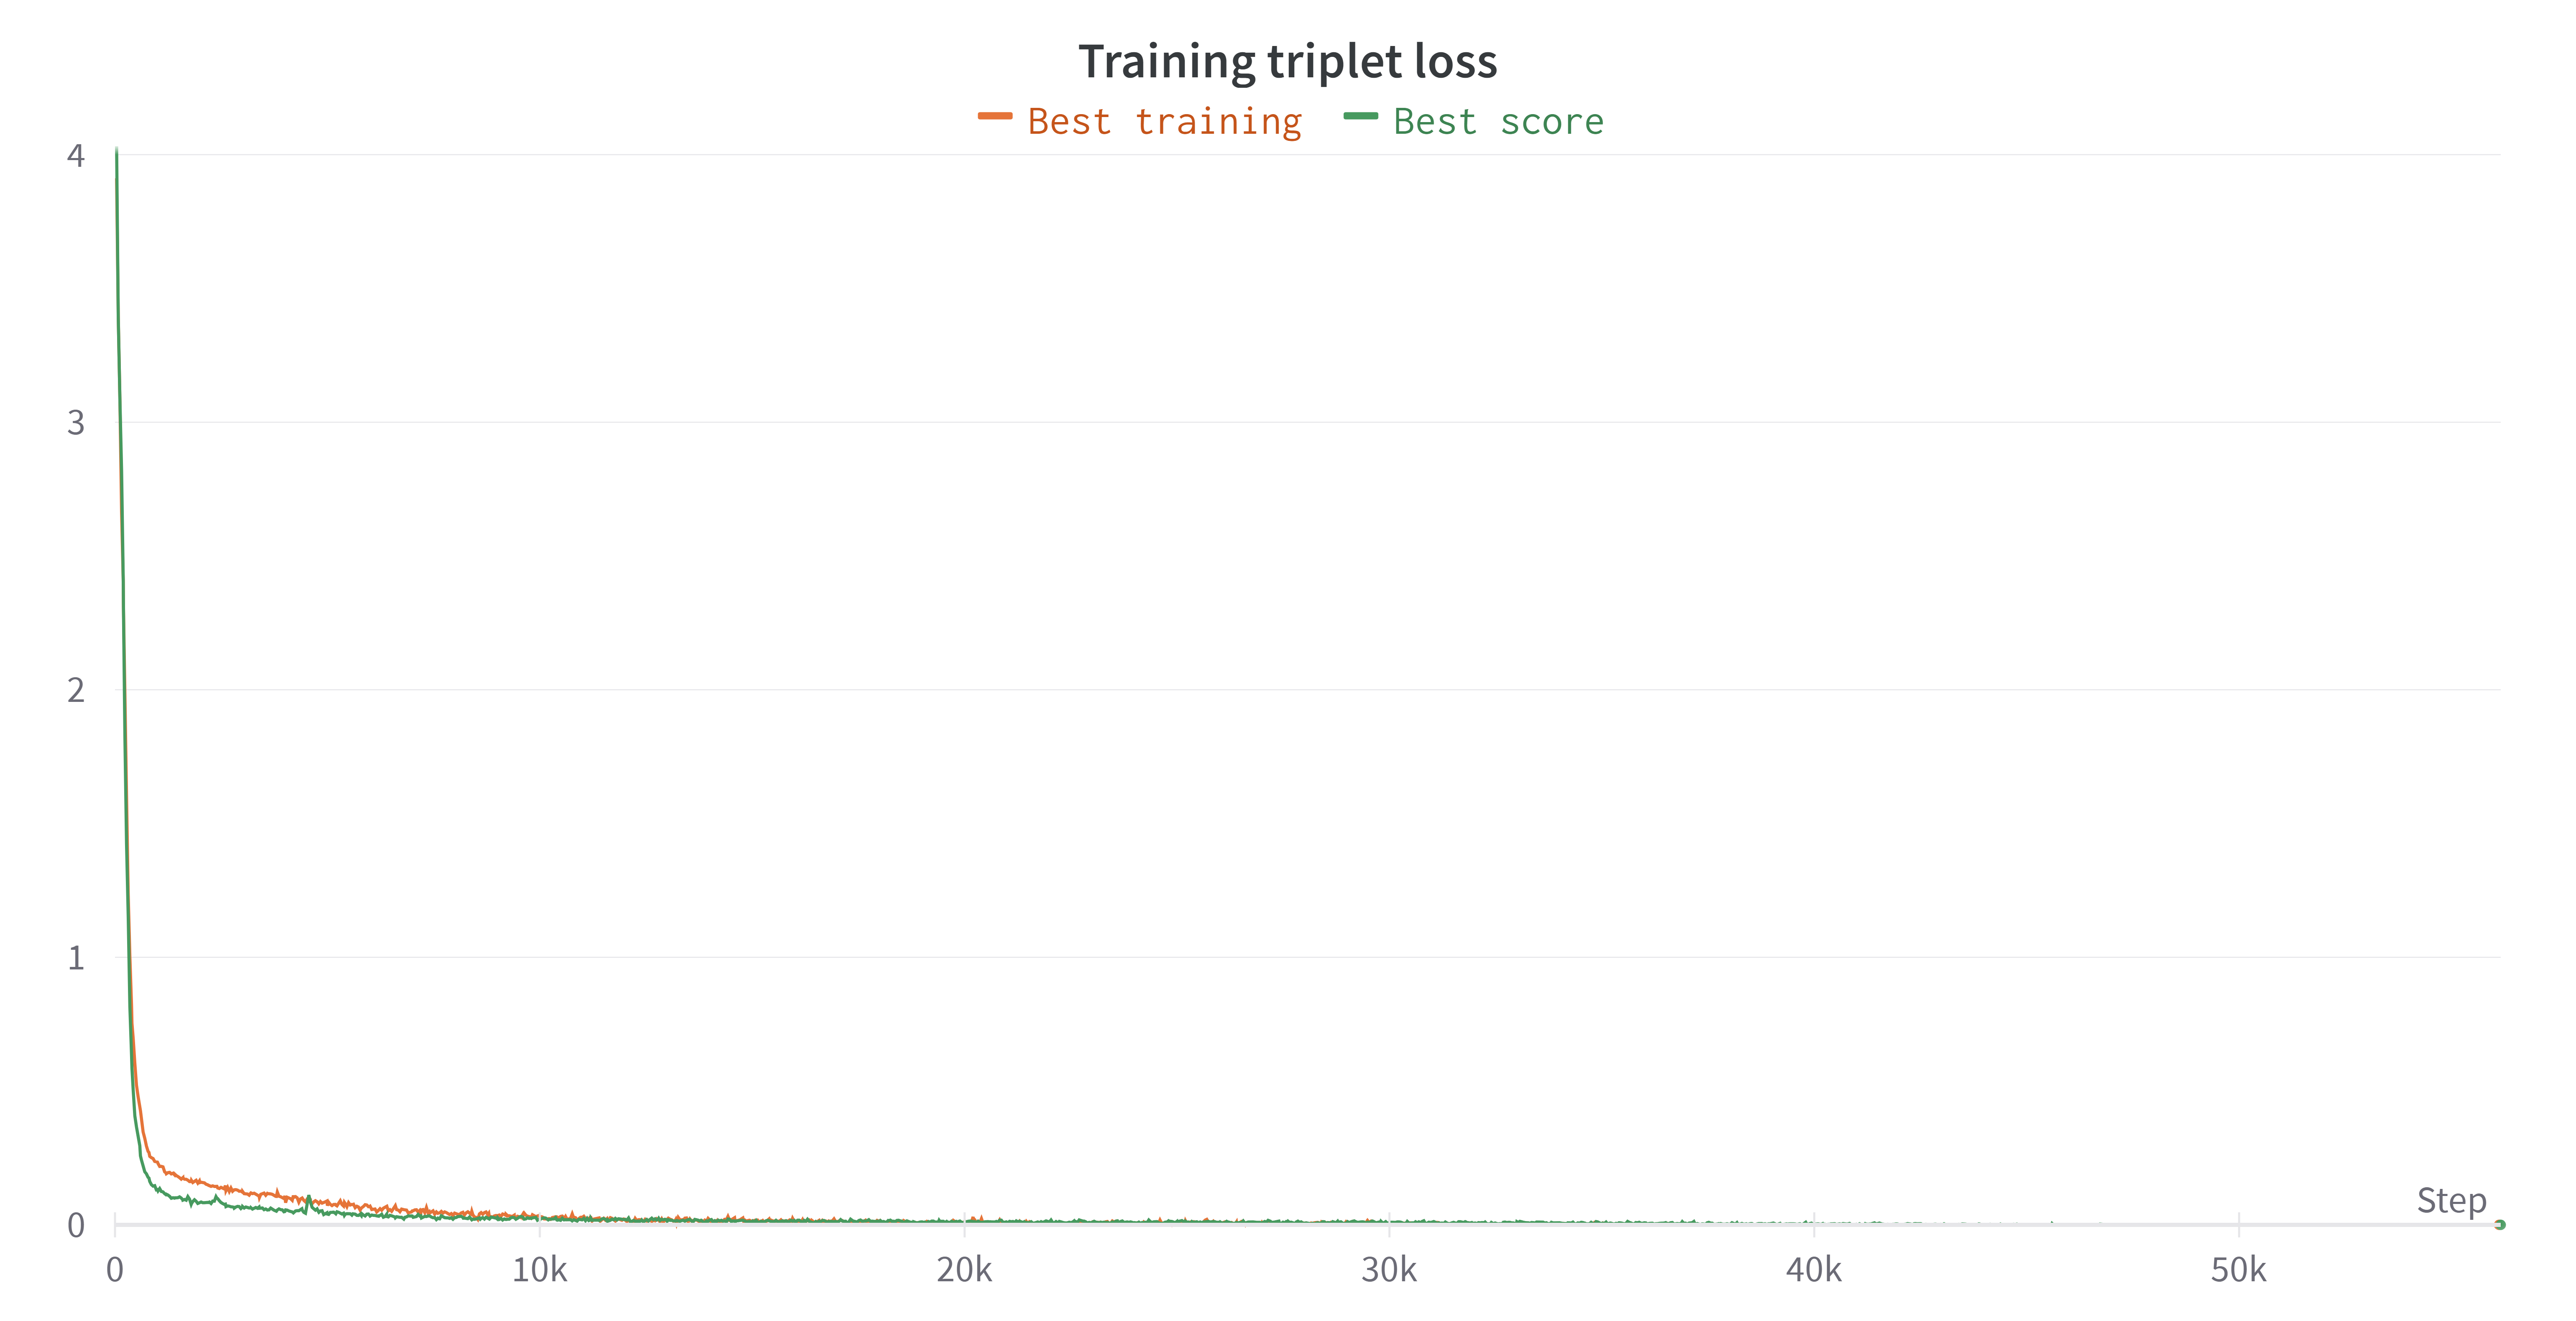
\includegraphics[width=\textwidth]{figures/06_results/ApperanceTrainTriplet.png}
		\caption{\footnotesize{Training triplet loss curve of BoT for two training settings.}}
		\label{fig:appearanceClass}
	\end{subfigure}
	\begin{subfigure}[]{0.9\textwidth}
		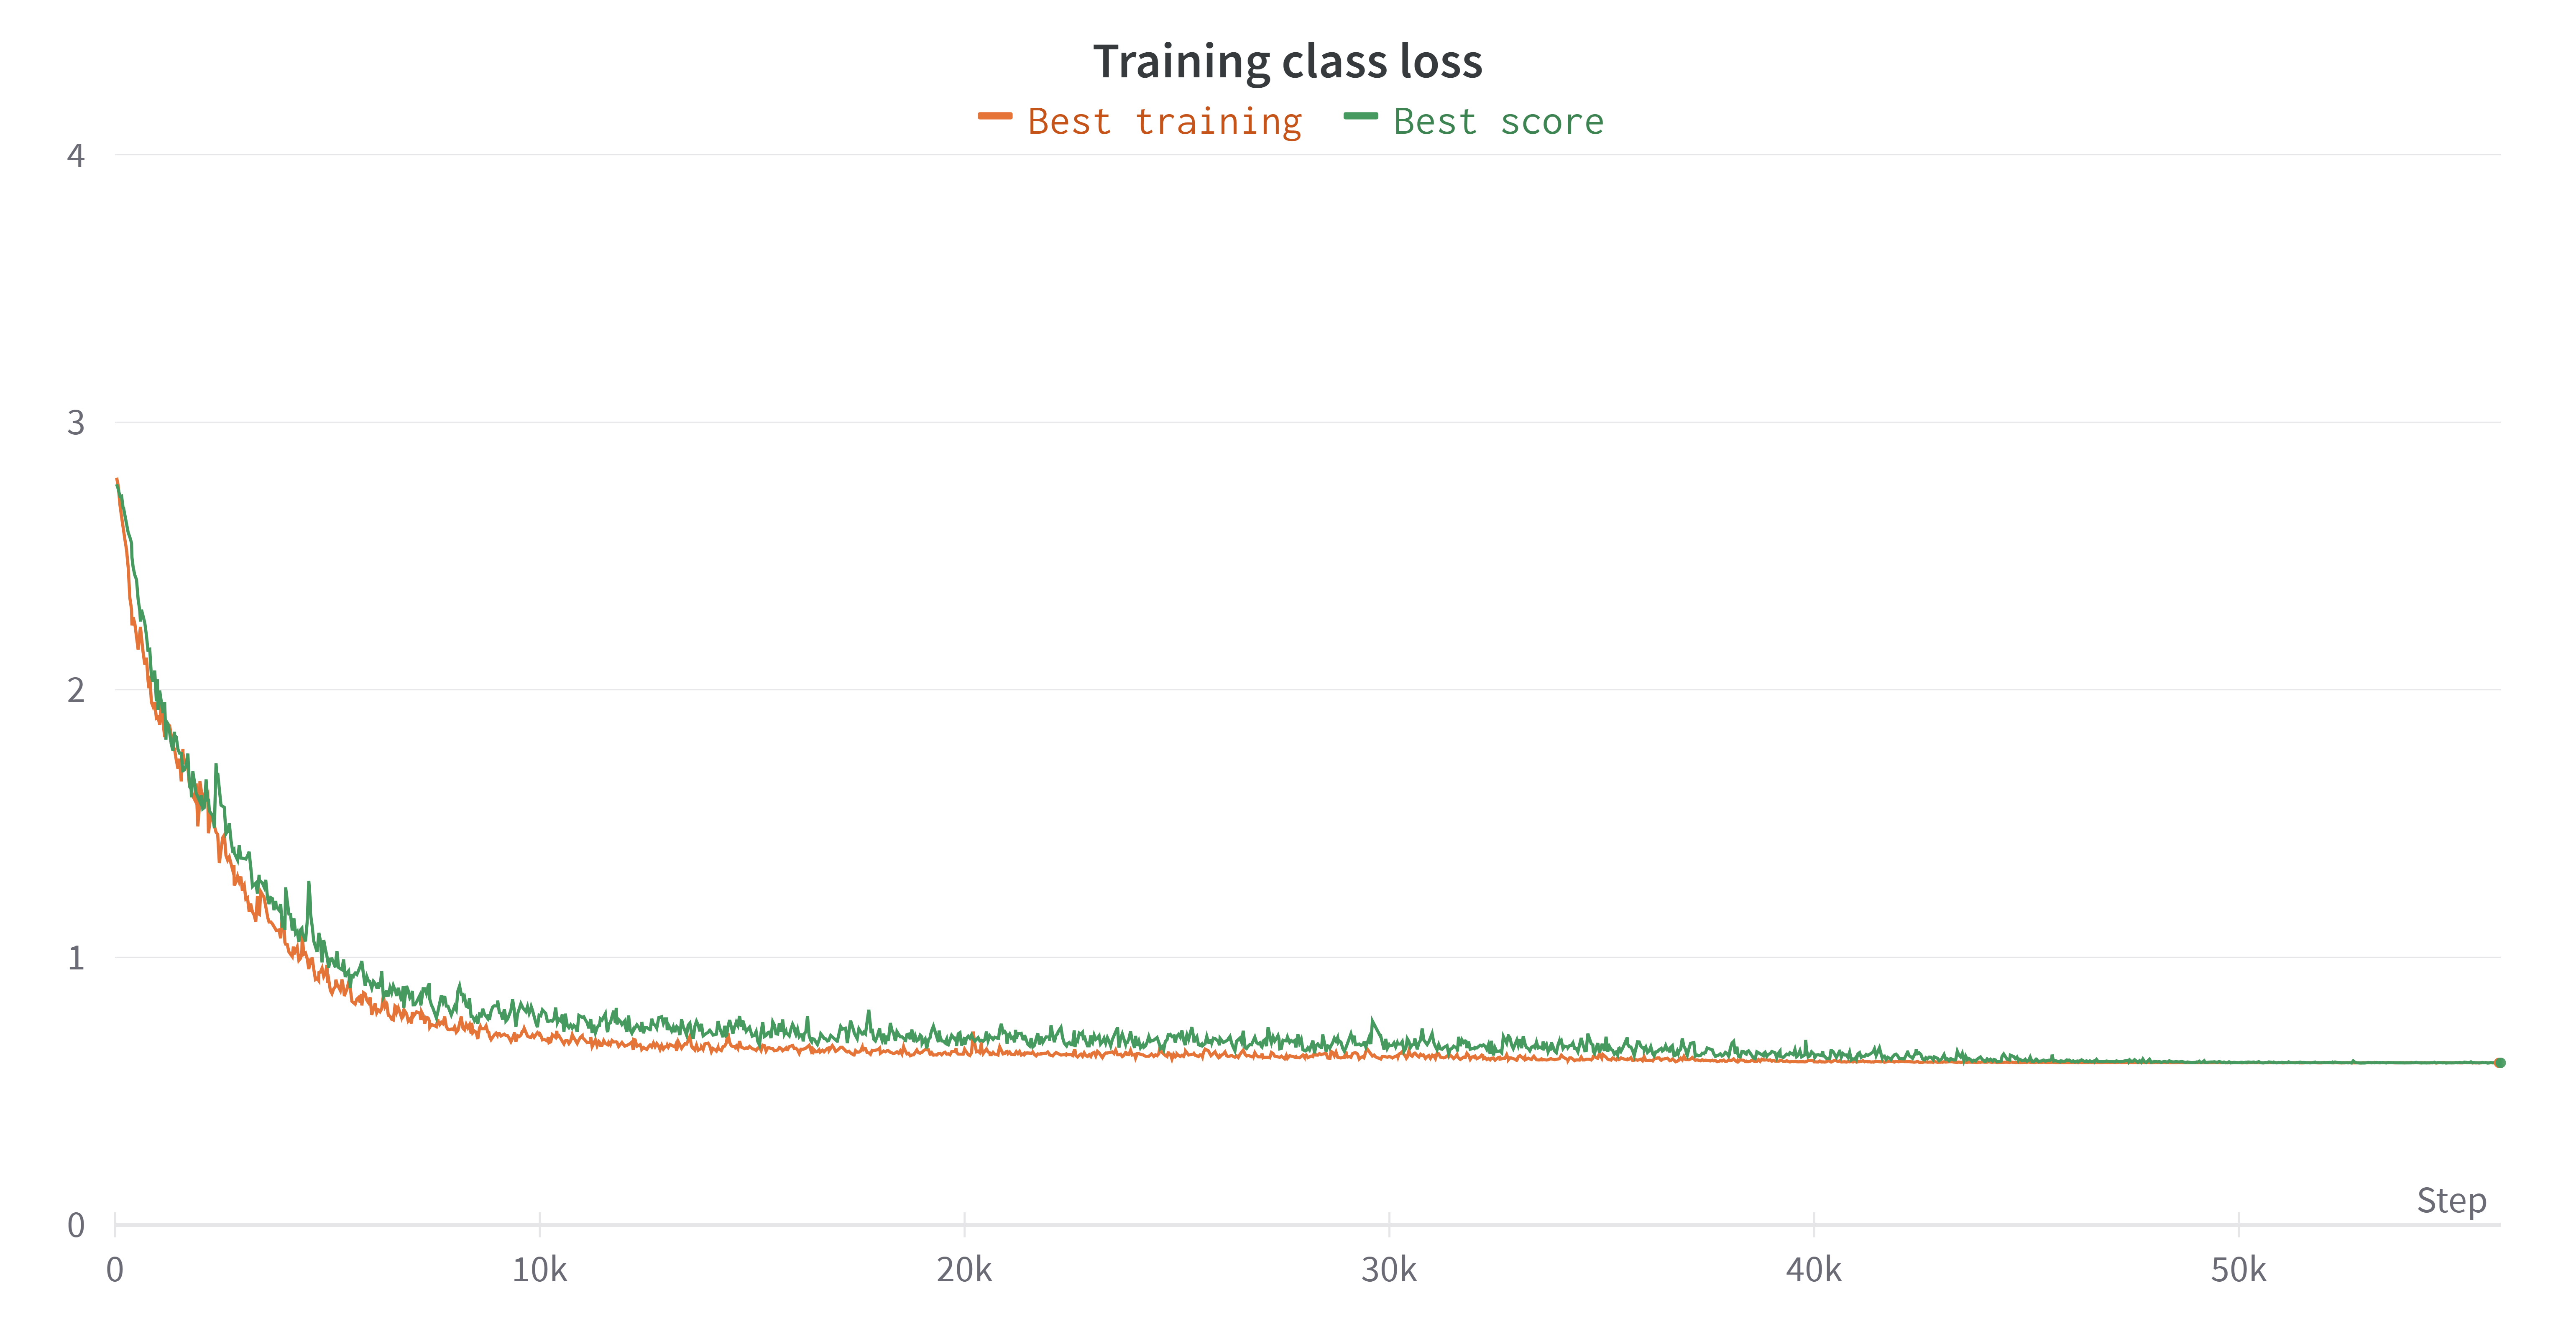
\includegraphics[width=\textwidth]{figures/06_results/ApperanceTrainClass.png}
		\caption{\footnotesize{Training classificationloss curve of BoT for two training settings.}}
		\label{fig:appearanceTriplet}
	\end{subfigure}
	
	\caption[Training Loss curves of BoT]{\footnotesize{Training Loss curves of BoT, it includes 2 training configurations.}}
	\label{fig:training appearance}
	\vspace{-4em}
\end{figure}

\begin{figure}[!p]
    \centering
    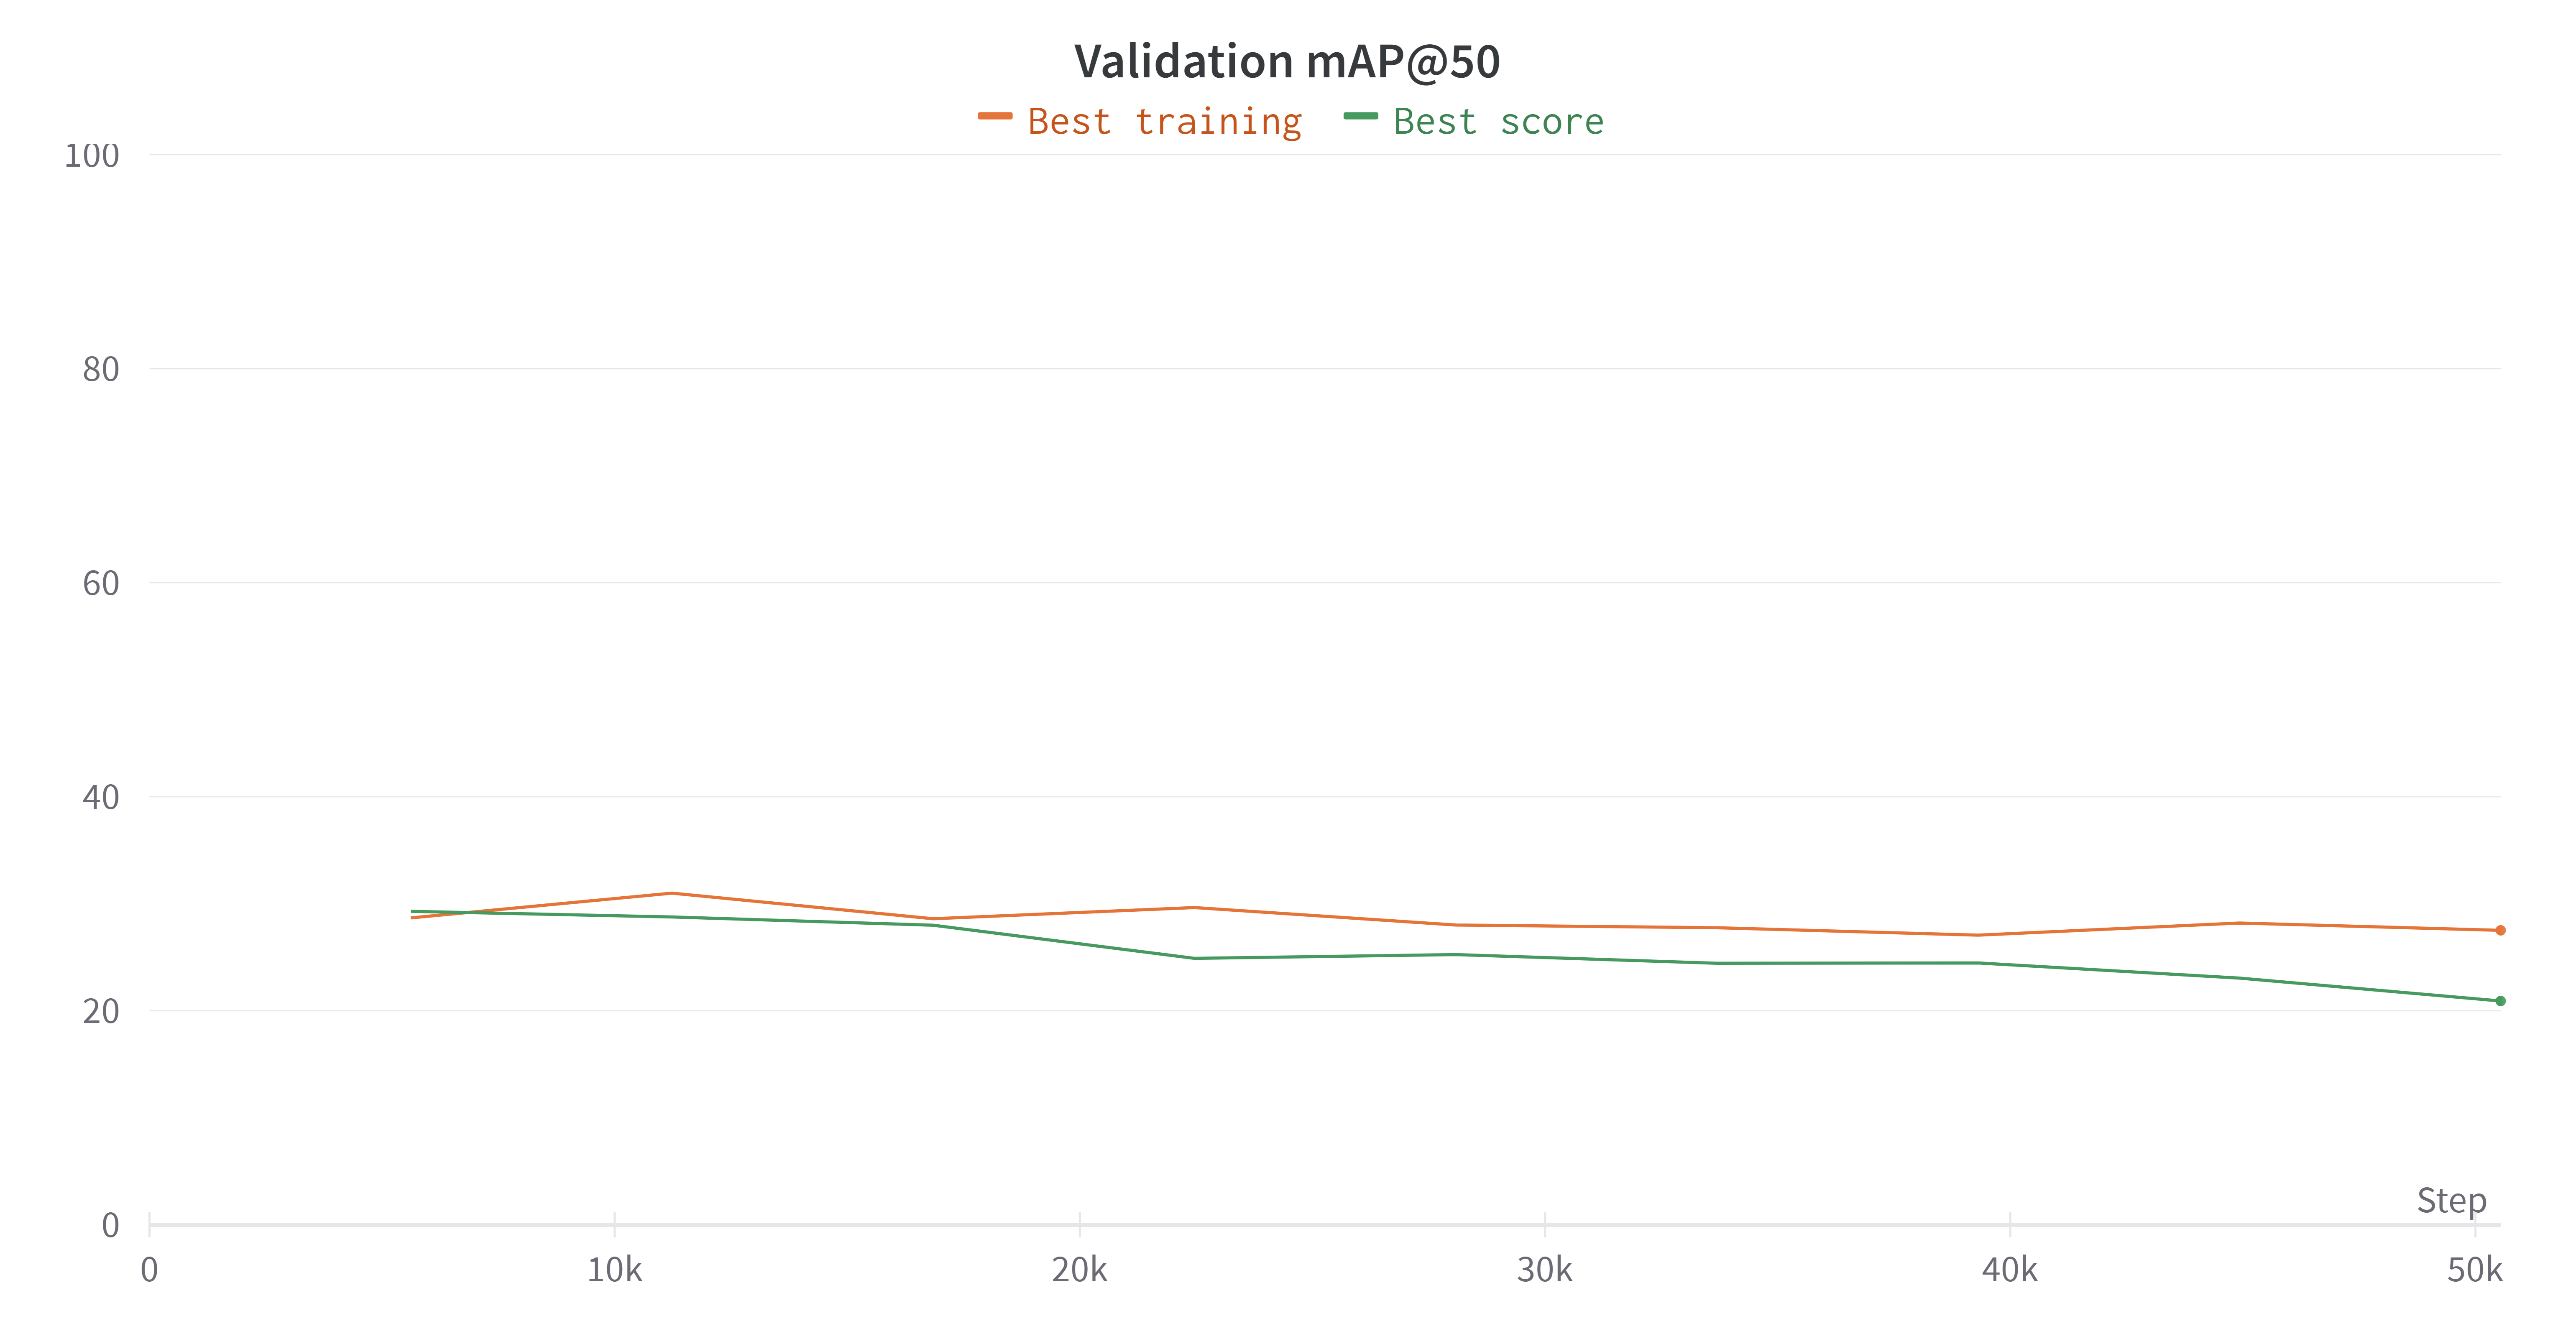
\includegraphics[width=0.9\textwidth]{figures/06_results/ApperanceValidationMAP.png}
    \caption[Validation mAP@50 curves of BoT]{\footnotesize{Validation mAP@50 curves of BoT for two training settings.}}
    \label{fig:appearance mAP50}
\end{figure}

\begin{figure}[!p]
	\centering
	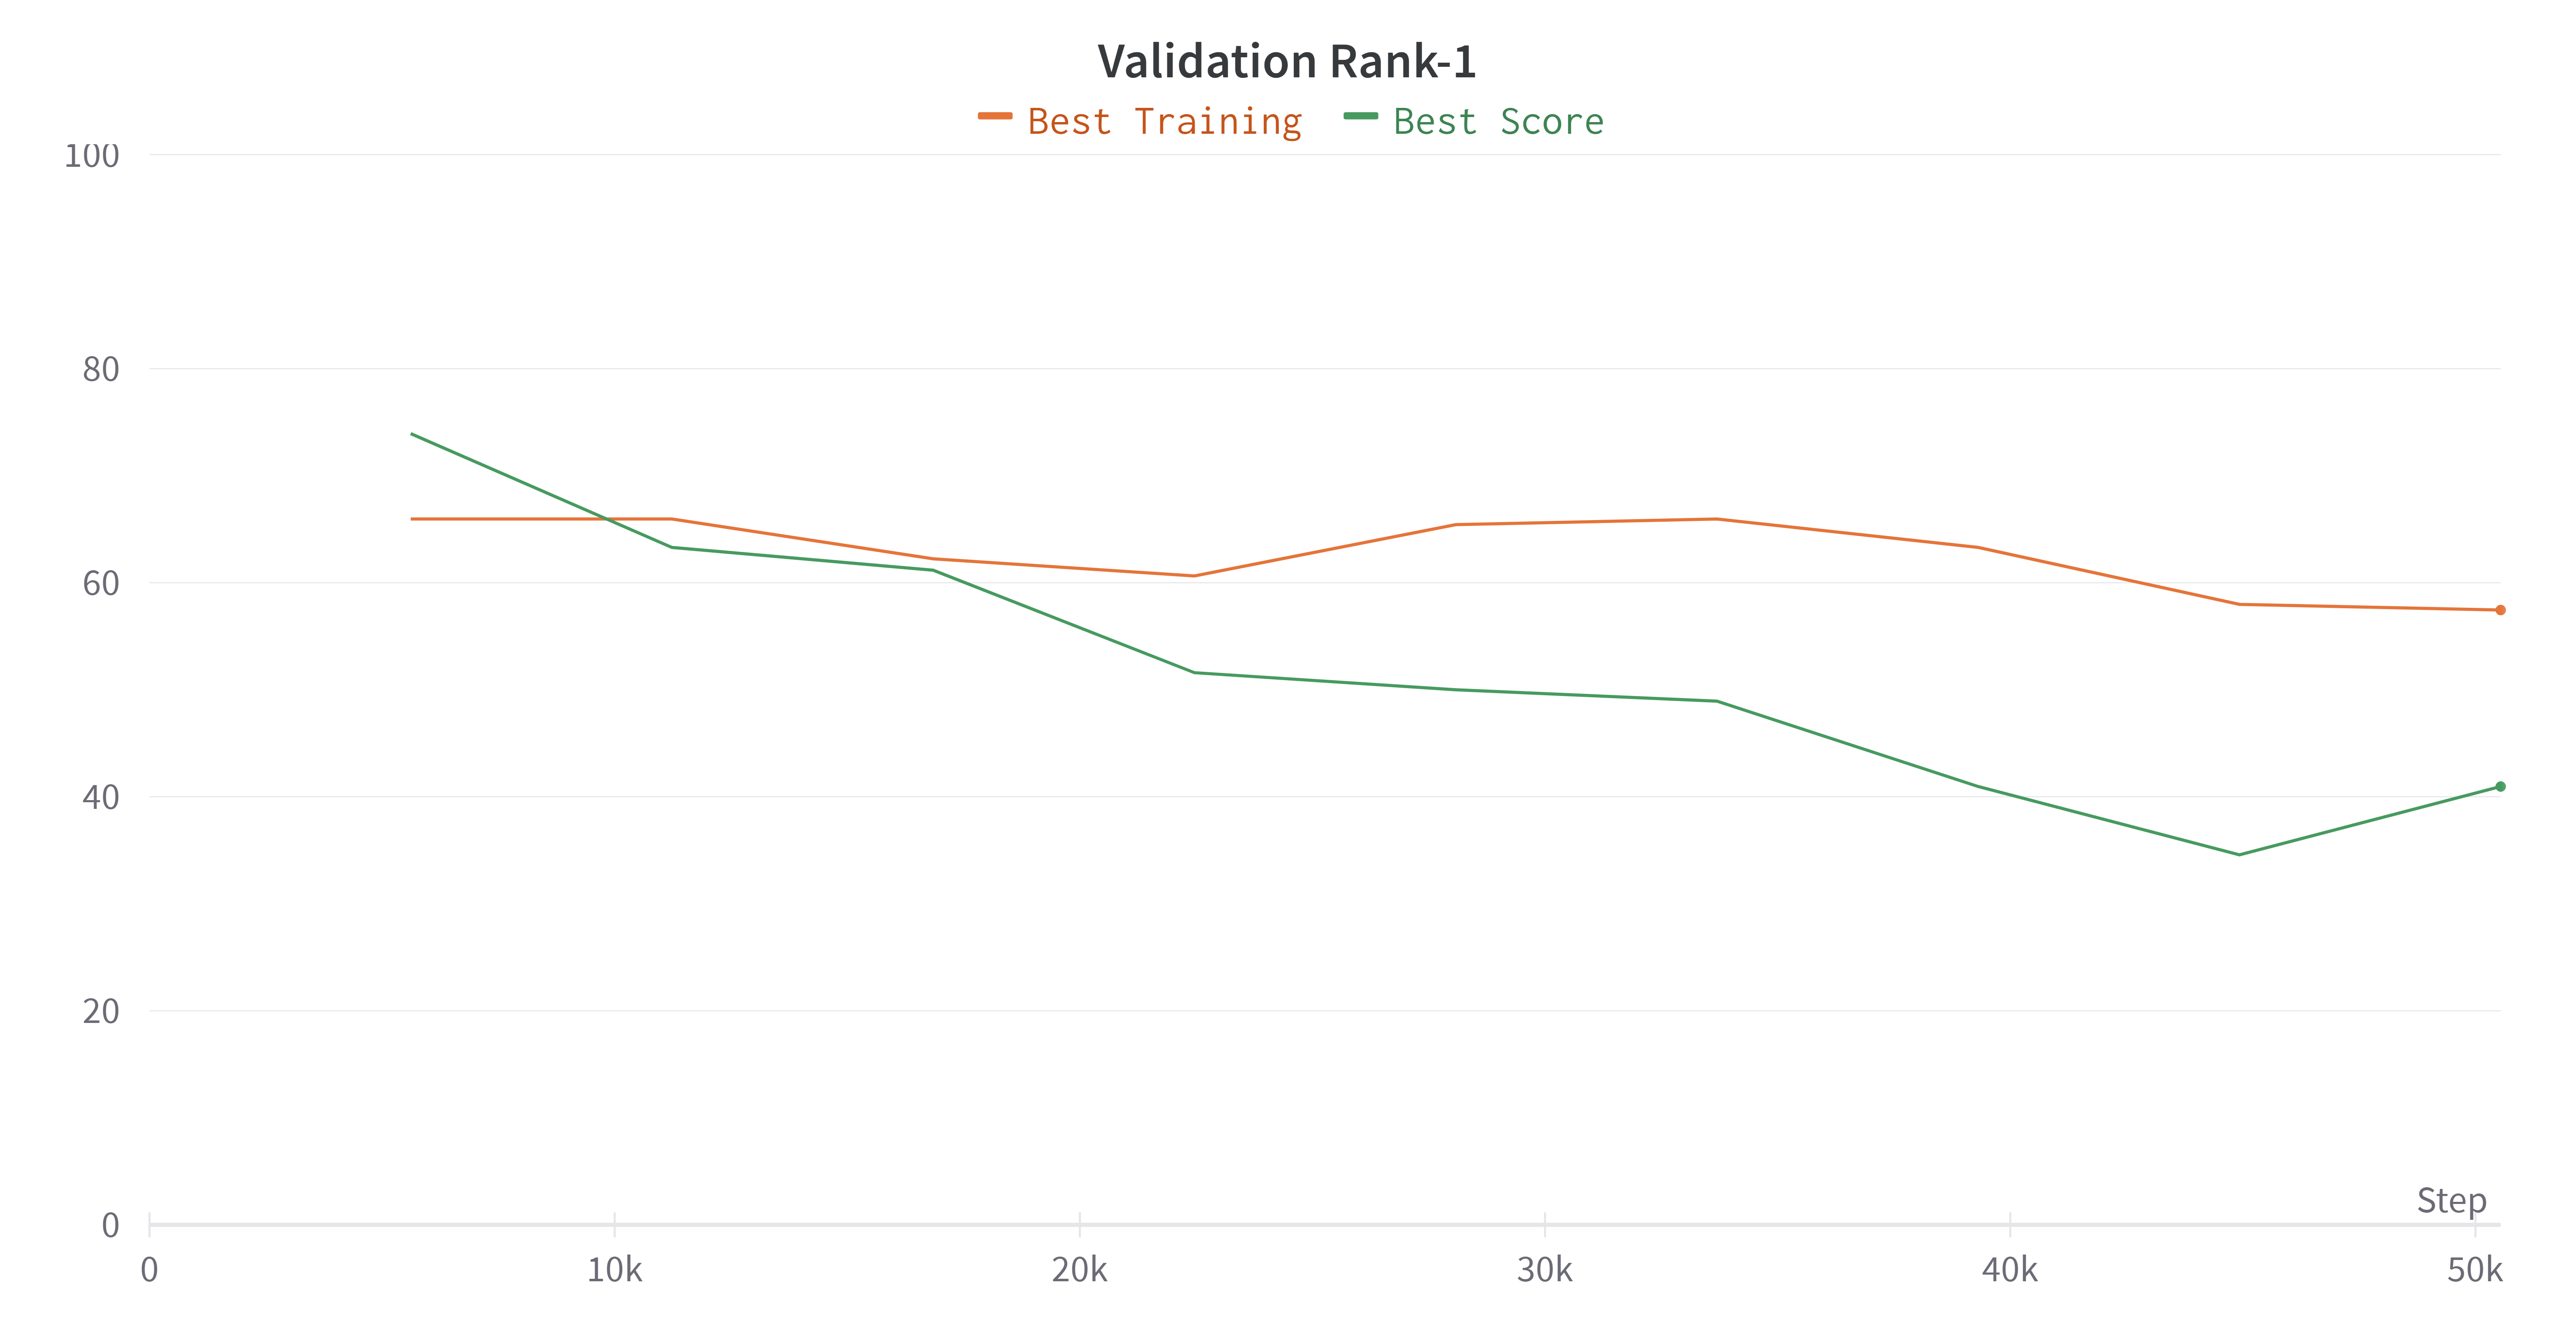
\includegraphics[width=0.9\textwidth]{figures/06_results/ApperanceValidationRank-1.png}
	\caption[Validation Rank-1 curve of BoT]{\footnotesize{Validation Rank-1 curve curve of BoT for two training settings.}}
	\label{fig:appearanceRank1}
\end{figure}
